%!TEX root = karulf-thesis.tex
\chapter{Implementation}

%% Unused!
% RIDE allows the human to increase or decrease the level of autonomy on a per robot basis. In contrast, the robots are capable of only decreasing the level of autonomy.

% Needs tightening -ek
%While the RIDE application does not specify any restrictions, I have elected to restrict the scope of my thesis to allow for a more careful examination of environmental searching within the range of supervised autonomy. In Section~\ref{section:futurework} I explain how these principles of RIDE could be adapted to support more autonomous behavior.


\section{User Interface}

The core of the RIDE user interface is the concept of sliding autonomy. In order to accomplish effective sliding autonomy, RIDE takes several cues from the video game industry. In our design phase, we decided to separate the user interface into two segments, the supervisor mode and the direct mode. The ``supervisor mode'' relies on robot to perform actions autonomously and report the information back to the human as appropriate. The ``direct mode'' allows the user to directly teleoperate a robot. By including both control styles, the user is given flexibility to use the most appropriate control mode for a given situation.

In addition to switching the control schemes between modes, we also change the fidelity of information exchanged. We found that providing streaming video for each robot was taxing not only on the network bandwidth but also on the human's perception. The movement from the video would draw the users eye to several places on the screen making effective management difficult. To combat this problem reduce the number of available sensors in the supervisor mode. When a user wishes to inspect a region with higher fidelity, switching into the direct mode enables all sensors for the current robot. This design decision seemed to be fairly intuitive as will be explained in Section ??.

\begin{figure}[ht]
\begin{center}
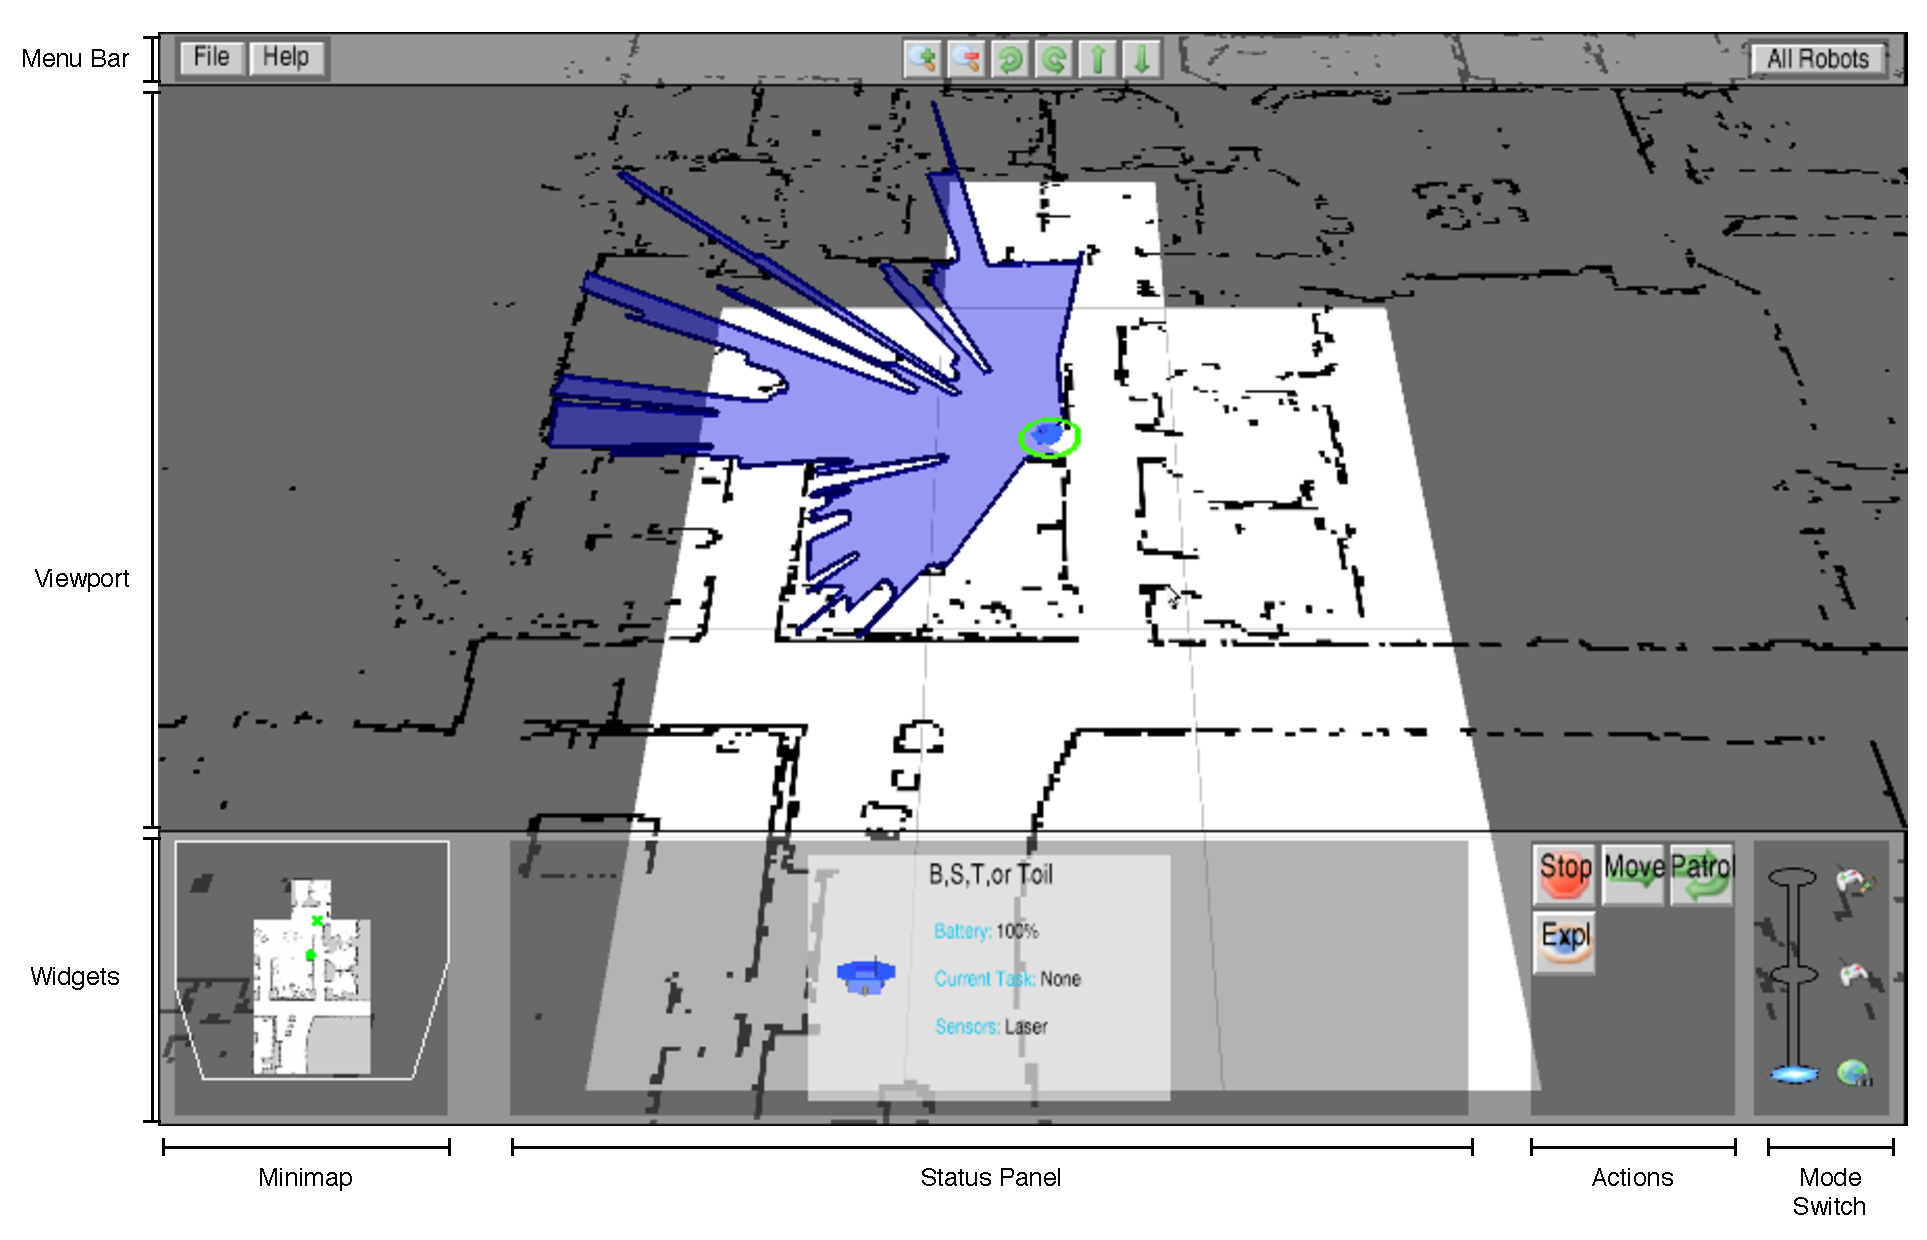
\includegraphics[width=6.10in]{images/ride-ui.pdf}
\caption{RIDE User Interface: Supervisory Mode\label{fig:ride-ui}}
\end{center}
\end{figure}

The screenshot figure in Figure~\ref{fig:ride-ui} shows the RIDE supervisory control mode with annotated descriptions of the user interface elements. The viewport is the main portion of the display. The viewport changes camera perspective based on the control mode, either locked behind the robot in the direct control mode or user operated in the supervisory interface. We took care to add alpha transparency to all user interface elements to prevent obstructing the viewport.

The menu bar at the top of the screen, remains static between the two control modes. The various menus allow for customization of the user-interface on a global and per-robot basis. These settings can be saved, and restored in future sessions. There are also menu bar buttons to control the camera viewpoint and zoom level, toggle the sensor information displayed, and to list all currently known robots.

At the bottom of the screen, the widget panel is displayed. The widget panel always contains a left, center, and right widget. A widget to change the display mode is always locked to the far right of the widget bar. Table~\ref{tab:ui-widgets} describes the widgets displayed based on the state of the interface.

\begin{table}[ht]
\label{tab:ui-widgets}
\begin{center}
    \begin{tabular}{ | p{4cm} | l | l | l |}
    \hline
    \textbf{Mode} & \textbf{Left Widget} & \textbf{Center Widget} & \textbf{Right Widget} \\ \hline
    Direct Control & Mini-map & Information Panel & Proximity Panel \\ \hline
    Supervisory Control (Single Robot) & Mini-map & Status Panel & Action Panel \\ \hline
    Supervisory Control (Multiple Robots) & Mini-map & Group Panel & Action Panel \\ \hline
    \hline
    \end{tabular}
    \caption{RIDE User Interface Widgets}
\end{center}
\refstepcounter{table}
\end{table}

\subsection{Supervisory Control}
\label{subs:ui-supervisor}

The supervisory control interface is what set's RIDE apart from the interfaces described in the prior work. Unable to find any large scale control interfaces within the realm of robots, instead we looked at the video game industry for inspiration. Our search led us to the genre of Real-Time Strategy games (RTS). 

As mentioned in Section~\ref{sub:RTS_games}, RTS games employ a top-down view of the world to control many units. We found that real time strategy games included their own task system. Furthermore, realtime strategy games support the control of heterogenous unit types; each unit type has separate abilities, strengths, and weaknesses. We wanted a way to visualize this information in the user interface without cluttering the main viewport during normal use. We developed two user interface widgets to represent the abilities, strengths, and weaknesses of each robot visually.

The first element known as the ``information panel'' can be seen in Figure ??. When a robot is selected, the information panel shows a listing of the robot's name, type, battery status, current task, and a list of sensors. A small 3D mockup of the front of the robot is also displayed to visually represent the make of the robot.

The second panel developed for the supervisory mode was the ``action panel.'' The action panel displays a list of buttons representing available actions for the selected robot. This list of actions is populated from what the robot self-reports actions it can perform. The implementation details of how actions are auto-discovered is briefly covered in Section ??. Clicking on a button will prompt for any additional arguments, such as asking the user to click on a position, and then send the task instruction to the robot. In our development we found that visualizing a confirmation helped improve clarity of what instructions were given to the robot. As an example when the user instructs a robot to move to a specific destination, the user interface will blink the target icon twice on the destination.  

In our study of RTS games, we found that players would organize units into heterogenous groups such that the individual units complimented each other's strengths and weaknesses. This required an interface that allows a user to select multiple robots at the same time and then command the group effectively.

When a user wishes to select a group of robots, instead of a single left click the user may left click and drag a rectangle around the robots he or she wishes to select. Much like single unit selection a detailed information panel will display relevant data about the robot. However, instead of showing detailed information on a single robot, the the ``information panel'' will be updated to show basic information on group as a whole. The information panel displays a 3D mockup for each robot currently selected and the name of the robot. The user may move the mouses on top of the 3D mockup to obtain additional information about the robot.

In addition to the information panel, the ``action panel'' also has a slight change in behavior. The action panel selects the union of set of actions available to each robot. RTS games provided a base set of actions that all controllable units must be able to perform, ``Stop'' and ``Move''. We require the same two actions to be available for all robots in RIDE. The advantage of requiring the move command for all robots is that we can use a shortcut found in most RTS games. When a robot is selected -- instead of click on the move button and then clicking on a destination, the user need only right click on the destination on the ground.

When porting the user interface from RTS games to human-robot interaction, we were able to re-use many of the existing design elements: unit selection, grouping, the action system, and mini-map. We also found that we needed to display additional elements: sensor visualization, coverage maps  decided to visualize additional sensor information when displaying robotic units. 


% Need more

% RTS view
% Higher concurrency / lower fidelity
% 
% \begin{figure}[ht]
% \begin{center}
% 
\includegraphics[width=3.5in]{images/placeholder.png}
% \caption{RIDE Supervisory Control\label{fig:ride-ui-super}}
% \end{center}
% \end{figure}
% 
% 
% % FPS view
% % Single concurrency / high fidelity
% 
% \begin{figure}[ht]
% \begin{center}
% 
\includegraphics[width=3.5in]{images/placeholder.png}
% \caption{RIDE Direct Control\label{fig:ride-ui-direct}}
% \end{center}
% \end{figure}

\subsection{Direct Control}

The direct control mode sets up a high fidelity of information exchange between the human and the robot as the user teleoperates the robot. Due to the large amount of prior work in the field of interfaces for teleoperation. We searched for video game design elements that would compliment the existing interfaces. While there are several styles of video game that we could draw on for inspiration, we decided to base our direct control mode off of ``open environment games.''

While not a genre in its own right open environment, or sandbox, games define a style of gameplay. Instead of the story following a predetermined linear path, the player is instead able to explore a world with the story unfolding around them. This style of gameplay is harolded by some as the future of games. Putting aside the narrative aspect of open environment games, the design elements that they employ have direct applicability to robotic interfaces.

The interfaces of open environment games are usually fairly minimal preferring leave most of the user interface available for camera display. The few user interface elements that do exist are typically semi-transparent to allow the user to see through UI components to the map. We applied this principal to all user interface components in RIDE by applying a small amount of alpha transparency. You can see an example of the transparency looking at the floor behind the user interface elements at the bottom of the screen in Figure~\ref{fig:ride-ui}.

In most open environment games, a third person camera follows behind the player's avatar. While controls exist that allow the user to manually rotate the camera, most gameplay occurs with default camera positioning. This camera control style is the inspiration behind our third-person direct control mode. The user uses the arrow keys on the keyboard to move the robot in a given direction and uses the mouse to rotate the camera as needed.

A common component of most open environment games is a minimap which allows users to orient themselves with relation to the ``world''. In video games, important characters, landmarks, and other notable locations may be displayed in the minimap. We added a minimap to the lower right hand corner of the RIDE user interface. The minimap is a component common to both the direct and supervisory control interfaces and we feel strongly that the minimap's location on screen should remain in the same location for both modes.

\subsection{Tasks and Notifications}
We adapted several elements from the Nielsen's ecological user interface in our design of RIDE. We designed the user interface to display inside a single viewport to avoid splitting the user's attention. We also procedurally construct a 3D world using the map and sensor data. This rich user experience allows the user visually perceive the state of the world as the robot perceives it. Finally, we introduced several new concepts to improve upon the weaknesses of the existing interfaces; a task system and a notification system.

We introduced an asynchronous task system allowing the human to directly command robots through a set of predetermined tasks. A robot may run only one single task at a time, and receiving a new task will replace the previous task. The task system was written generically to allow each robot to provide actions appropriate to its hardware and software. Additional details on the implementation of the task system can be found in Section~\ref{subs:ui-supervisor}.

To complement the task system, a notification system was also introduced. The notification system allows the robot to communicate with the human. The design of the notification system was enables the robot to select the importance of the message, and it permits the human to filter messages by importance. This gives the human operator the ability to ignore routine informational messages while still receiving urgent messages. An example notification is shown in Figure~\ref{fig:ride-notification}. The example shows the robot self-reporting that it has discovered a box, it's goal in this search and rescue scenario.

\begin{figure}[ht]
\begin{center}
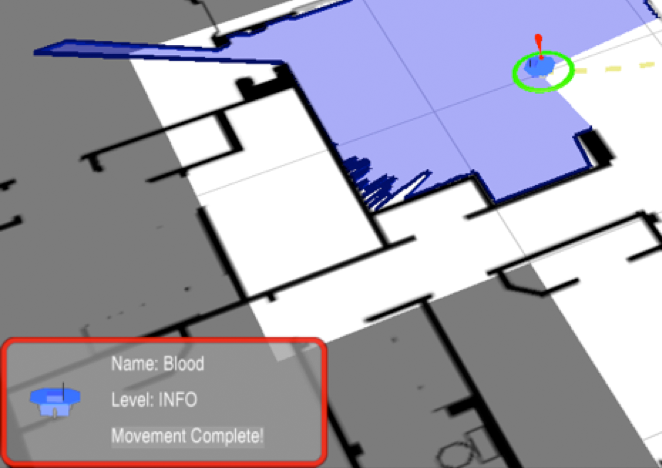
\includegraphics[width=6.10in]{images/ride-notification.png}
\caption{RIDE Notification Example\label{fig:ride-notification}}
\end{center}
\end{figure}


\section{Robot Operating System}
The Robot Operating System (ROS), developed by Stanford University and Willow Garage, is a specialized adaptation of the Common Object Request Broker Architecture (CORBA) design pattern for robotics software. This design decision gives ROS a modern distributed architecture that encourages small, reusable code.

The ROS architecture can be thought of as a directed graph. Software components are called ``nodes'' and are run in separate processes. This allows each node to be written using the most appropriate language to the task. As an example, a performance sensitive node could be written in C while a less demanding node could be written in Python for improved readability. At the time of writing ROS supports C++, Python, Java and Lisp.

% Nodes => Package
% Pacakages => Stack
% Stack => Repositories

\subsection{Topics and Services}
ROS provides a framework for connecting nodes together. Nodes can be connected together through a ``topic'' or through a ``service''. A topic is a named stream that supports multiple readers and writers. Nodes that write to a topic are known as ``publishers''. A publisher announces that it is publishing to one or more topics to the ``roscore'' node. 

The ``roscore'' node is a special node that is run when the ROS environment is initialized. It acts as a directory server maintaining a list of active nodes, topic, services, and configuration values.

Nodes that wish to read from a topic are known as ``subscribers''. Similar to publishers, a subscriber will announce it is listening to one ore more topics to the roscore node.

The roscore node continually informs subscribers of the location of publishers. This allows nodes to communicate directly without needing to contact the roscore node. Currently only TCP and UDP unicast sockets are supported, however future releases of ROS will include shared memory and multicast networking. A simple example of a ROS digraph can be seen in Figure~\ref{fig:middleware-ros}.

\begin{figure}[ht]
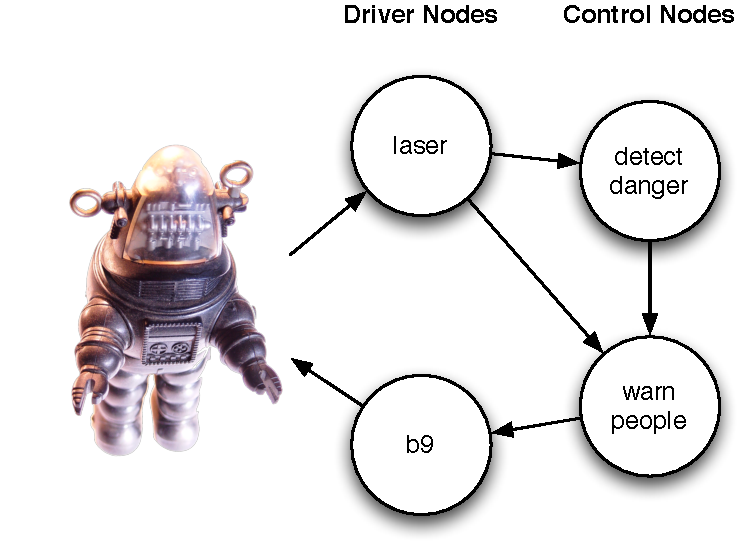
\includegraphics{images/middleware-ros.pdf}
\caption{Example ROS application\label{fig:middleware-ros}}
\end{figure}

The development of nodes can build on each other. Low-level hardware interface nodes communicate raw sensor and actuator messages. Unlike traditional robotic driver software, ROS allows the developer to break the control code up into several pieces. This modular interface allows code re-use of control code as well as driver code.

% TODO: correct acronym IDL
ROS also defines a common message format for communicating. Messages are defined using a independent-domain language (IDL) which in turn auto-generate serialization and deserialization code for supported languages. An example message file can be seen in Figure~\ref{fig:point}.

\begin{figure}[ht]
\makebox[\textwidth]{\hrulefill}
\begin{verbatim}
	# This contains the position of a point in free space
	float64 x
	float64 y
	float64 z
\end{verbatim}
\makebox[\textwidth]{\hrulefill}
\caption{Point.msg : Message representation of a 3D Point\label{fig:point}}
\end{figure}

\subsection{Kinematic Tree}
A large part of the complexity of robotic systems is transforming coordinate frame in a timely manner. ROS offers a special topic located at \verb!tf! and provides a cross-language library, also called ``tf'', to ease coordinate transformation tasks.

ROS builds a kinematic tree using data published to the \verb!tf! topic. Coordinate frames contain a timestamp, an object's name, the parent coordinate frame and the quaternion offset between the two. The tf package allows a developer to request a quaternion offset between two coordinate frames. 

In order to maintain a correct representation, the library automatically discards stale coordinate frame data. This requires objects to publish their location at a specified frequency. When all nodes are publish at an acceptable rate the full kinematic tree is accessible. A sample kinematic tree for a robot with a stero-vision rig mounted on-top of a pan-tilt unit can be seen in Figure~\ref{fig:tf-example}.

\begin{figure}[ht]
\begin{center}
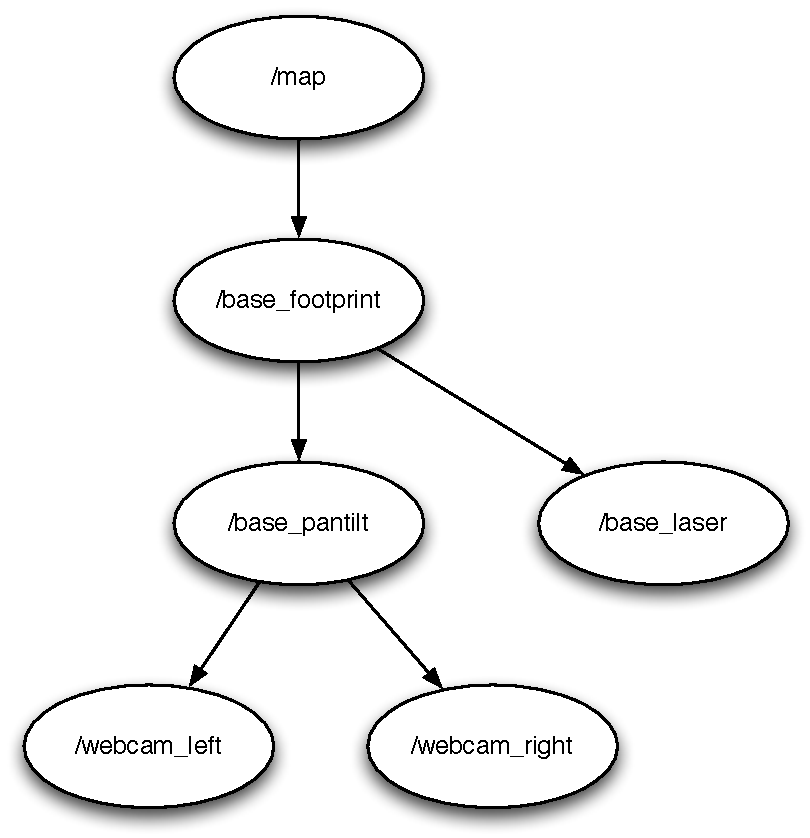
\includegraphics[width=3.5in]{images/tf-example.pdf}
\caption{Sample Kinematic Tree\label{fig:tf-example}}
\end{center}
\end{figure}

\section{RIDE Architecture}

ROS was originally designed for a single robot system. A node may only be attached to a single ROS graph (or ``realm''). RIDE is designed to work with large numbers of robots. Early on in the development cycle, I decided to stick to the model that realms are local to a robot. This allows robots to operate independently of connectivity to eachother, and does not require any changes to existing single-robot code bases. This design conflict required the development of a new node library called ``rosmultimaster''.

rosmultimaster allows a single node to connect to multiple realms using the native ROS python (rospy) codebase. rosmultimaster is multi-threaded library that provides both a synchronous and asynchronous interface. Further implementation details for rosmultimaster can be found in Appendix X % TODO: Appendix number

Using the rosmultimaster code-base, we developed RIDE to connect to each robot on startup, as well as a single mapping realm. A high level overview can be found in Figure X.X. The map realm acts as a central location to for map retrieval / updating. In the future, if ROS were to support peer-to-peer networking, a map could be dynamically built by stitching together several independent maps. 

% TODO: Generate high level figure

\subsection{Simulation Realm}
\label{sub:simulator}
I used a simulation environment, called ``rosstage'', to provide a consistent environment. The simulated system architecture is a superset of the regular RIDE architecture with the map realm acting as a full simulation realm and several additional topics being shared to the robot realms. An overview of the simulation architecture can be found in Figure~\ref{fig:ride-simulation-realm}.

\begin{sidewaysfigure}[ht]
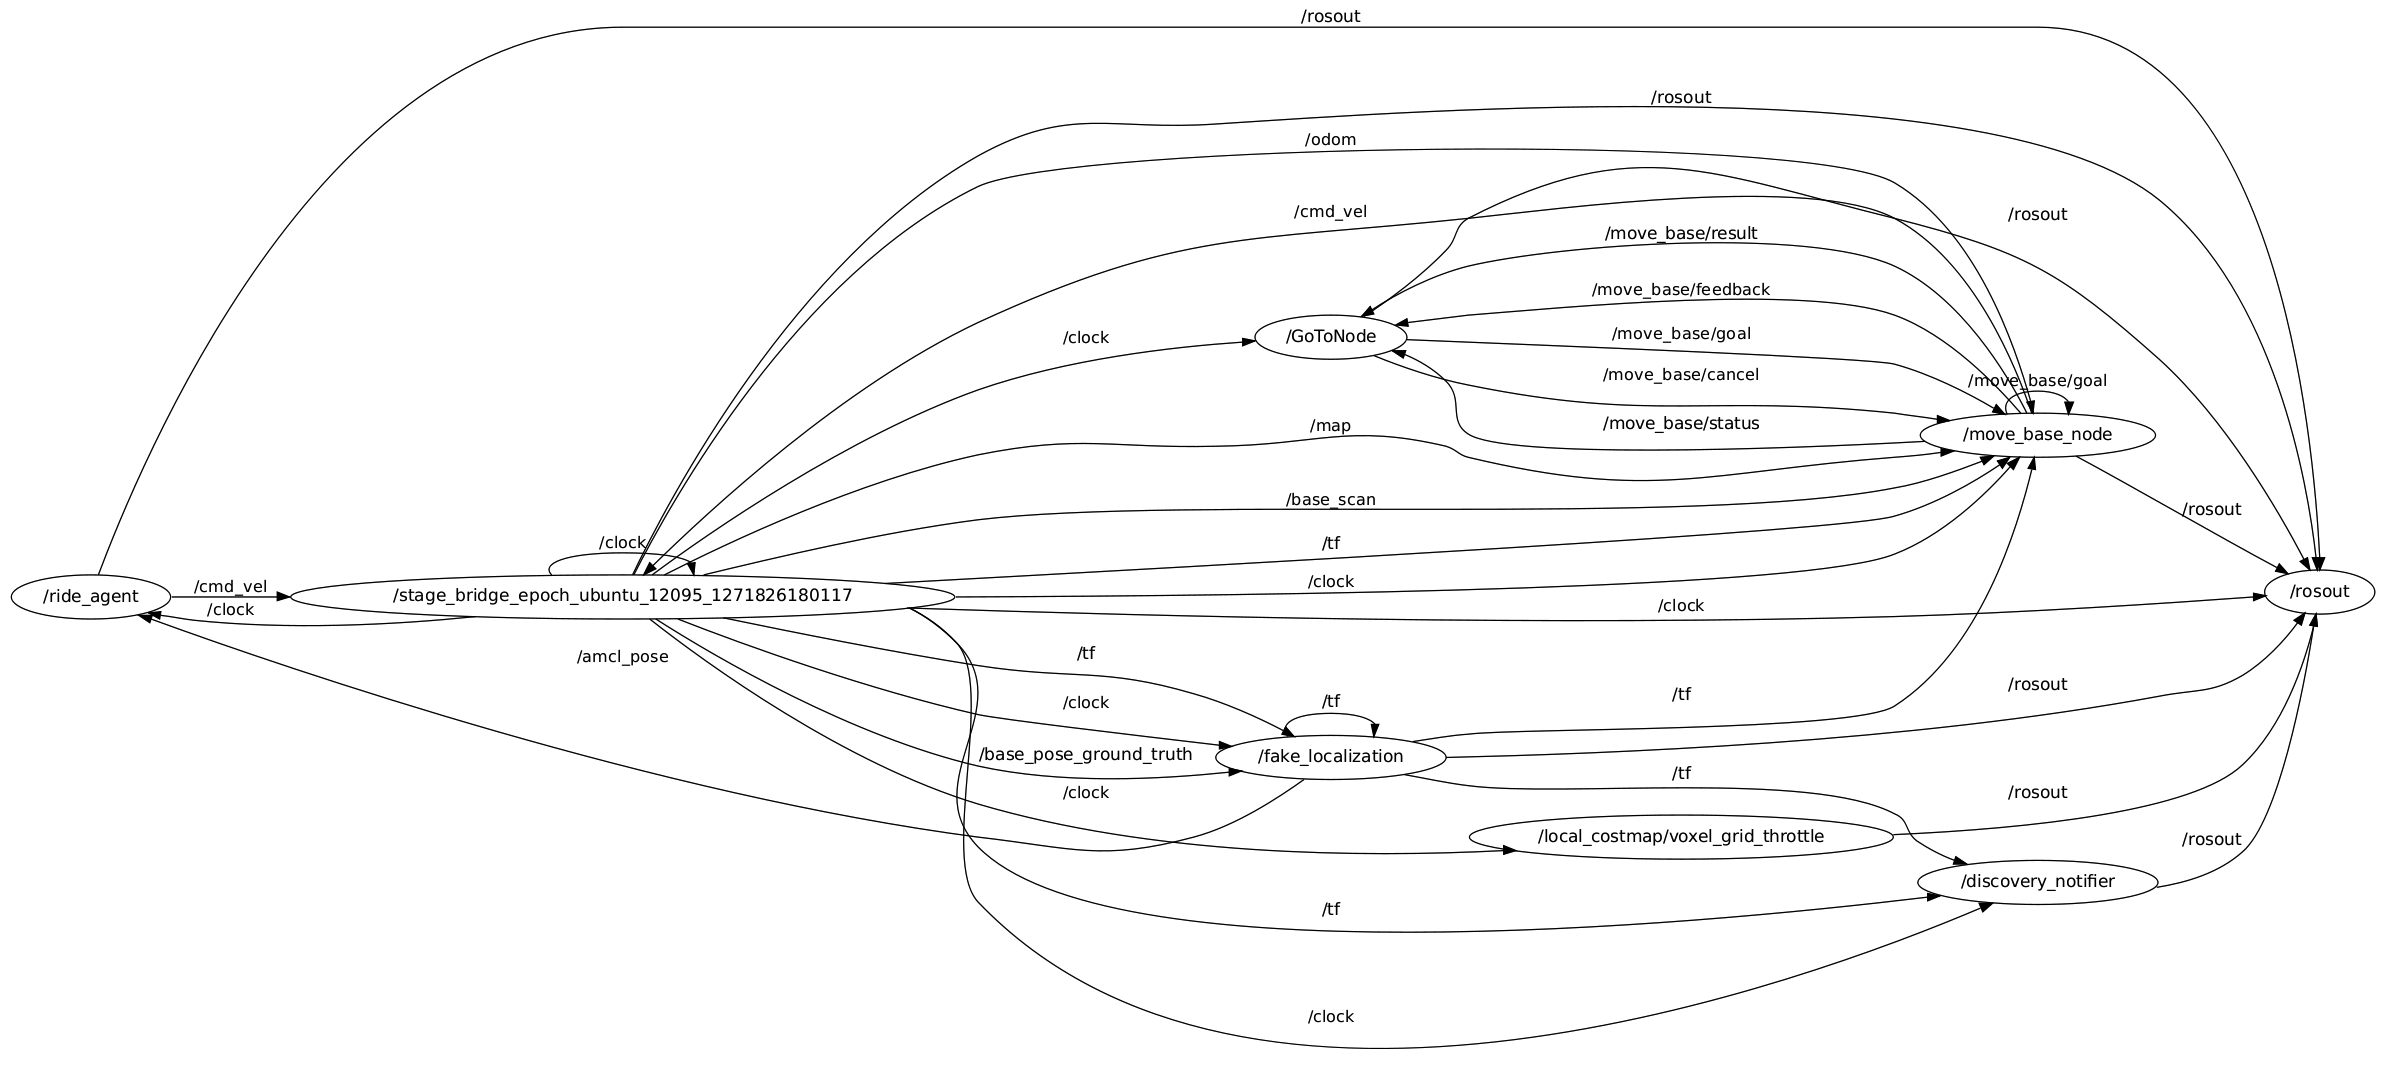
\includegraphics[width=\textwidth]{images/ride-simulation-realm.png}
\caption{Publish/Subscriber graph in RIDE Simulation Realm\label{fig:ride-simulation-realm}}
\end{sidewaysfigure}

\subsection{Robot Realm}
\label{section:robot-architecture}
RIDE uses a modular structure for controlling robots. Due to the topic system in ROS, this functionality can be written to work regardless of if the robot is simulated or physical. Each robot must provide position data for basic RIDE functionality. Beyond position data, the user can choose what sensors, actuators, and ``actions'' to provide.

Figure~\ref{fig:ride-robot-realm} demonstrates a simulated robot realm and the components to the most basic functionality. The robot must be able to orient itself with respect to the \verb!/map! coordinate frame. This typically requires a localization node like the Adaptive Monte-Carlo Localization (amcl) node when running on a physical robot or a fake localization node when running in simulation.

In addition to providing position data, the robot must expose a path planning node. ROS provides a navigation stack complete with a path planning node, called move\_base. Lastly, the robot must provide a way to directly control the movement of the robot allowing the user to ``drive'' a robot around freely.

% Discuss ride_agent
% Discuss GoToNode

\subsection{Panda3D Integration}

RIDE uses the popular 3D rendering engine Panda3D to display the virtual environment to the user. Panda3D is implemented in C++ for performance reasons, and provides a Python interface that we used to integrate with ROS. 

Like most rendering engines, Panda3D relies on a scene graph for rendering objects onto the screen. We kept a one-to-one mapping of objects in ROS's kinematic tree to objects in Panda3D's scene graph. This natural mapping proved to be simple and effective.

We developed a simple configuration file, using the YAML format, to let users configure which realms RIDE should connect to and what models to use when rendering objects from ROS's kinematic tree in the Panda3D scene graph. An example can be seen Figure~\ref{fig:tf-example}, where a single robot contains a laser range finder. Future work would remove the configuration file, moving the connection information into the user interface, and updating the RIDE protocol to provide dimensions and model information as needed.

% TODO: Insert figure: RRS / scene graph

Panda3D provides its own run loop for running tasks, processing events and updating the scene graph. For performance reasons, Panda3D does not use the native Python threading implementation so I chose to use the synchronous API offered by rosmultimaster. I then added one background task per rosmultimaster instance to Panda3D's task manager. The rosmultimaster tasks were called at a specified frequency designed to keep latency low and framerate high.
